% !TEX root = ../TAMU_Thesis_Main.tex

%%%%%%%%%%%%%%%%%%%%%%%%%%%%%%%%%%%%%%%%%%%%%%%%%%%%%%%%%%%%%%%%%%%%%%
%%                           SECTION I
%%%%%%%%%%%%%%%%%%%%%%%%%%%%%%%%%%%%%%%%%%%%%%%%%%%%%%%%%%%%%%%%%%%%%

\chapter{Introduction and Literature Review}

\section{Author's Message to the Student Using This Template For Their Thesis or Dissertation}

Howdy! This is the template for theses and dissertations written using \LaTeX for submission at Texas A\&M University. While the \ac{OGAPS} is here to guide you in submitting your thesis or dissertation. This template shows the many features of \LaTeX, with many more available to the user.

Please note that this is NOT the official template supported by \ac{OGAPS}. If you have issues, please submit an issues on the github page or email me at wodzicki [at] tamu [dot] edu.


\subsection{Brief Usage of the Template}

This template is intended for use by STEM\footnote{Science, Technology, Engineering, and Mathematics. This is an example of a footnote. You can see that it is numbered and appended at the end of the page. Also, you can see the effect of having a multiline footnote.} students. If you are not a STEM student, this template is likely not for you.

The advantage of using this template over the Microsoft Word templates are numerous. First, there is a lot of control granted to the user in how the document looks. Of course, you are expected to still follow the guidelines set forth in the TAMU Thesis Manual. This template takes care of the margins, heading requirements, and front matter ordering for you.


\subsection*{Software to Install}

\textbf{MikTeX} or \textbf{ProTeXt} is the free software recommended for Windows PC users to
compile their \LaTeX ~ document. \textbf{MikTeX} is also available for Mac OS X users. To compile for this document, XeLaTeX compiling engine is used. There is currently an issue in which the package xetex-def does not install; see the file README.txt for a solution. Another software called \textbf{JabRef} is also recommended for bibliography/reference management; its usage is similar with EndNote.

\subsection*{Procedure to Compile \LaTeX\ Document}

This template (and consequently, your document) will be compiled using XeLaTeX. To compile your document, do the following\footnote{Notice here that I also show off the itemize environment for unordered lists. Ordered lists use the enumerate environment.}:

\begin{itemize}
	\item In TeXstudio, go to the Tools menu, then select Commands, and click XeLaTeX.
	
	\item In Texmaker, go to the Tools menu and select XeLaTeX.
	
	\item For other editors, consult the help files included with the editor.
\end{itemize}

To view the output after the program is done compiling, press F7 in TeXstudio and TeXmaker or the appropriate hotkey for other editors. Be sure that the document is not open in another PDF reader, for your editor will not display it.

\subsection{How to Fill This Document}
The document structure is organized in the main .tex file, TAMU\_Thesis\_Main.tex,
which has the same name as the output PDF file. Content in each section is in the Data folder. You can open the .tex files under the data folder to modify. Four sections
are added initially. To add in more sections into the \LaTeX document, open the
TAMU\_Thesis\_Main.tex file and go to the section that says ``Include all chapters/sections of the thesis'' and include more .tex files.

\section{Reference Usage and Example}

As previously mentioned, one program that can be used to organize references is \href{http://www.jabref.org}{\textbf{JabRef}}. While a tutorial of how to use \textbf{JabRef} is beyond the scope of this template, a brief discussion of how to use \textbf{BibTeX} follows.

\subsection{BibTeX}
After you have installed \textbf{JabRef}, or any citation manager of your choosing that is compatible with \textbf{BibTeX}, you must create a \textbf{BibTeX} database. This database file will contain all the information \textbf{BibTeX} requires to generate your bibliography. An example .bib file named `myReference.bib' is included in this template. The first entry of that file is shown below.\footnote{The example of a BibTeX entry also shows the `verbatim' environment, where text is displayed in monospaced font in the exact format that it is typed in the .tex document.}

{\footnotesize \begin{verbatim}
@Article{Barn-JORVQ,
  author  = {Christopher F. Barnes and Richard L. Frost},
  title   = {Residual Vector Quantizers with Jointly Optimized Code Books},
  journal = {Advances in Electronics and Electron Physics},
  year    = {1992},
  volume  = {84},
  pages   = {1--59},
}
\end{verbatim}}

All of the keys in the bibtex entry are very self-explanatory, such as author and title, however, arguably the most important part of the entry is the key. The key is the first value after @Article, which is Barn-JORVQ in this example. This is the key you will use in any cite commands for references, e.g.,

\begin{verbatim}\cite{Barn-JORVQ}\end{verbatim}

which will give you the following when used in text \cite{Barn-JORVQ}. If you used a different key you will get the number, or author/year depending of citation style, that corresponds to that citation \cite{REALCAR}. You can also use multiple keys in one cite command, just separate them using commas \cite{ANCONS, WAGFJ, einstein}. If you happen to use an undefined key, or just simply spell it wrong by mistake, you will get a question mark as follows \cite{notdefined}.

Depending on the citation style that is used, there may be different cite commands for different types of in-text citations. It is important to know which commands must be used with the citation style you are using.

\subsection{Compiling with BibTeX}
When compiling your \LaTeX{} document with {\bf BibTeX} citations, four different compiles must be done to ensure that all references are updated correctly. This entails running XeLaTeX, then BibTeX, then XeLaTeX twice. This will ensure that all the citations and cross-references are updated correctly. If you are using a program such as \textbf{MikTeX} or \textbf{ProTeXt}, this may be the default compilation method. However, if you use \textbf{TeXShop} on a Mac, you must change the compiler manually. If compiling from command line, the sequence would be:

\begin{verbatim}
xelatex TAMU_Thesis_Main.tex
bibtex TAMU_Thesis_Main.aux
xelatex TAMU_Thesis_Main.tex
xelatex TAMU_Thesis_Main.tex
\end{verbatim}

Note that {\bf BibTeX} must be run on the .aux file, not the main .tex file. Be sure to check the output for any errors. If question marks (?) appear in any location where a reference should be, there was an issue with the compilation. Make certain that the key used in the cite command matches the corresponding references in the .bib file.

\subsection{References at the end of chapters}
If you would like references at the end of each chapter, first make sure you are using the `chapref' options in the documentclass command at the top of the main \LaTeX document. Once that option is set, compilation is similar to the method discussed above.

First, compile the main file use XeLaTeX. When it is done compiling, check the directory your document is saved in. There should be a bunch of files named `bu*.aux', where the asterisk represents any number. You will now want to run {\bf BibTeX} on all of these .aux files as well as the .aux file from the main document. After {\bf BibTeX} is run on all the .aux files, run XeLaTeX two more times and your document should be good to go! If you are on a Mac, open up a Terminal window, cd into the directory your document is in and run the following commands (should work on any Linux machine as well):

\begin{verbatim}
xelatex TAMU_Thesis_Main.tex
find ./ -name '*.aux' -exec bibtex '{}' \;
xelatex TAMU_Thesis_Main.tex
xelatex TAMU_Thesis_Main.tex
\end{verbatim}

The second command simply finds all the .aux files in the current working directory and executes (exec) the command bibtex on each of them.

Be sure to check the output for any errors. If question marks (?) appear in any location where a reference should be, there was an issue with the compilation. Make certain that the key used in the cite command matches the corresponding references in the .bib file.

\section{Acronyms, Equations, Formulas, and Other Really Cool Math Things That \LaTeX\ Can Do}
\subsection{Acronyms}
Using acronyms (or nomenclature) in \LaTeX\ is great because it keeps track of which acronyms have been used throughout the document. In the case of the template, that is done through the nomenclature package\footnote{The nomenclature package in this distribution uses the acro package to handle the acronyms and the longtable and tabu packages for formatting the nomenclature section of the document.}. By default, the nomenclature package is loaded in the {\it TAMU\_Thesis\_Main.tex} file just after the documentclass command with the {\it all} option enabled. With the {\it all} option set, all acronyms/nomenclature defined in the {\it nomenclature.tex} file will appear in the Nomenclature section of the document. If you want only those acronyms used in the document to appear in the Nomenclature section, remove the {\it all} option from the package loading. If you would like the long form of acronyms/nomenclature to appear when hovering over the short version in text, add the {\it hover} option when loading the nomenclature package.

To edit the acronyms and nomenclature for the document, open up the {\it nomenclature.tex} file in the the Data directory. Below is the entry for the OGAPS acronym
\newpage % Force new page

{\small \begin{verbatim}
\DeclareAcronym{OGAPS}{
	short   = OGAPS,
	long    = Office of Graduate and Professional Studies,
	list    = Office of Graduate and Professional Studies at Texas A\&M University,
	tooltip = Office of Graduate and Professional Studies
}
\end{verbatim}}

The {\it DeclareAcronym} command sets up a new acronym, with the first argument (in this case OGAPS) being the key used to access the acronym. After this, we define some attributes of the acronym. The {\it short} key defines the short version of the acronym. In this case, it is the same as the acronym key, OGAPS. The {\it long} key defines the full definition of the acronym that will appear in text, in this case Office of Graduate and Professional Studies. The {\it list} key defines how the acronym will be defined on the Nomenclature page. As you can see, this is different from the long version that will appear in the text. The last key is {\it tooltip}. This sets the definition that will appear when hovering over the short version of the acronym in the text if the hover option is set when loading the nomenclature package. Let's show some examples.

To use an acronym, is the {\it ac} command, or the {\it acp} command for a plural form (adds `s' to end). For example: {\it ac}: \ac{OGAPS}, {\it acp}: \acp{OGAPS}. Notice that \ac{OGAPS} was not defined in the text. That is because it was already defined at the beginning of the document. This means, you do not have to remember which acronyms you have already defined, just use the {\it ac} command whenever calling an acronym. You can also explicit access the long and short forms of the acronym: {\it acs}: \acl{TAMU}, {\it acl}: \acs{TAMU}. Note that these commands change the `used' state of the acronym, so future calls of {\it ac} produce only the short form: \ac{TAMU}. If you would like to reprint the definition, you can use {\it acf}: \acf{TAMU}. A final useful command is {\it acresetall}. This resets the `used' state for all acronyms to unused. This might be useful to use at the beginning of a new chapter so that all acronyms will be redefined in the new chapter. For more acronym definition and use options see the documentation for the acro package\footnote{\url{http://mirror.hmc.edu/ctan/macros/latex/contrib/acro/acro_en.pdf}}.

\subsection{Equations}
Equations can be written in \LaTeX ~ in one of two ways. First, you can have material displayed inline by enclosing the desired statement in dollar signs. For example, $e^{i\pi}+1=0$ is an inline math expression. Some longer expressions, especially those including sums, integrals, or large operators and objects can be displayed centered on their own line. In this \textbf{math mode}, you enclose the desired material in square brackets. For example,

\[ \sum_{j = 1} ^n \int f_j \ dx = \int \sum_{j = 1} ^n f_j \ dx \]
is a math mode expression. We can also have a series of expressions aligned at a symbol. This is particularly useful when you are showing details in solving an equation or evaluating an integral. The next block shows off the \textit{align*} environment. We use it here to show a distributive property of set intersections over unions. Observe how each line is aligned to the biconditional symbol. This makes reading steps easier, since a reader can go line by line and determine why each step is justified.

\begin{align*}
x \in A \cap \bigcup_{j} B_j &\iff x \in A \ \wedge \ x \in \bigcup_{j} B_j \\
&\iff x \in A \ \wedge \ x \in B_k \ \text{ for some k} \\
&\iff x \in \bigcup_{j} A \cap B_j
\end{align*}

Some more information about equations appears in Section \ref{sec:more_equations}\footnote{This is an example of a cross-reference to a section. You can use the {\bf label} command to label just about any point in the document; in this case I labeled the 'Equation' section in Chapter 2 with the label `sec:more\_equations'. You can then use the {\bf ref} command with the label to get the exact chatper.section.subsection.etc, with all the information updating automatically as chapters/sections are added removed.}.

%Have some material about the align environments. Include also the eqn environment.

\section{Specifications in This TAMU \LaTeX ~ Template}

All requirements for theses can be found in the most recent version of the Thesis Manual, available at the \ac{OGAPS} website. The Thesis Office will be happy to assist you if you have questions about formatting\footnote{Remember that this is NOT the official OGAPS \LaTeX template}.

A common question students ask is the placement of a copyright statement at the beginning of a section with reprinted material from a previously printed source. The screenshot below describes how to achieve this. Check the instruction files for more details.

\begin{figure}[ht!]
\centering
	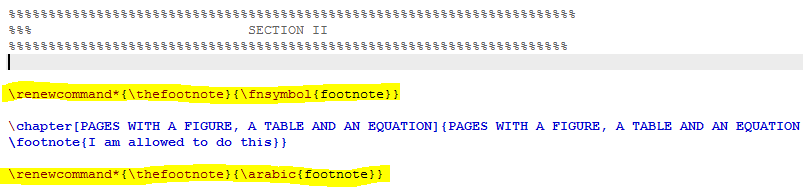
\includegraphics[scale=0.65]{Footnote.png}
	\caption{The inclusion of a copyright statement as a footnote. The lines in yellow help to change to footnote marking scheme.}
\end{figure}